
\section{General vRNIC interface}
In native RDMA, the application accesses RNIC by the Verbs interface. Correspondingly, we presents uniVerbs interface, which is general to containers and virtual machines. Moreover, the interfaces have strong isolation and are transparent to all RDMA applications. At the same time, uniVerbs interface maps RDMA resources bewteen RDMA applications and vRNICs for zero copy and bypassing the virtual layer.
	
\subsection{Basic uniVerbs Interface Construction}
The RDMA applications in containers and virtual machines are both the processes of host. Therefore, the general interface are avialable for both containers and virtual machines. 

For containers, vRNIC can be directly provided to RDMA applications in containers by IPC(inter-process communication). However, for virtual machines, the vRNIC in the host user space and the RDMA application in the virtual machine user space are separated from the emualted hardware environment and the guest operating system. Therefore, it is necessary to use I/O virtualization technology to extend each vRNIC as an I/O device of the virtual machine. Then, driver for this device must be installed in virtual machine to support the I/O process. Therefore, the uniVerbs interface for the virtual machine includes two following works:

\begin{itemize}
\item {\verb|Extend vRNIC as I/O device|}: 
The existing I/O virtualization technologies are mainly divided into full virtualization and paravirtualization. The full virtualization completely simulates all the functions of the device, there are frequent context switching and data copy overhead. 
In contrast, paravirtualization does not emulate the hardware complemently to reduce the times of data copy and switch. Therefore, we exploit paravirtualization to expand vRNIC as an I/O device. In our design, the I/O channel between vRNIC and the virtual machine is a shared memory queue, which is created by file; the signal and interrupt mechanism can be realized through the event descriptor between virtual layer process and each virtual machine process, then the event notification is converted into an internal interrupt signal by virtual machine monitor.
 
\begin{figure}[!ht]
	\centering
	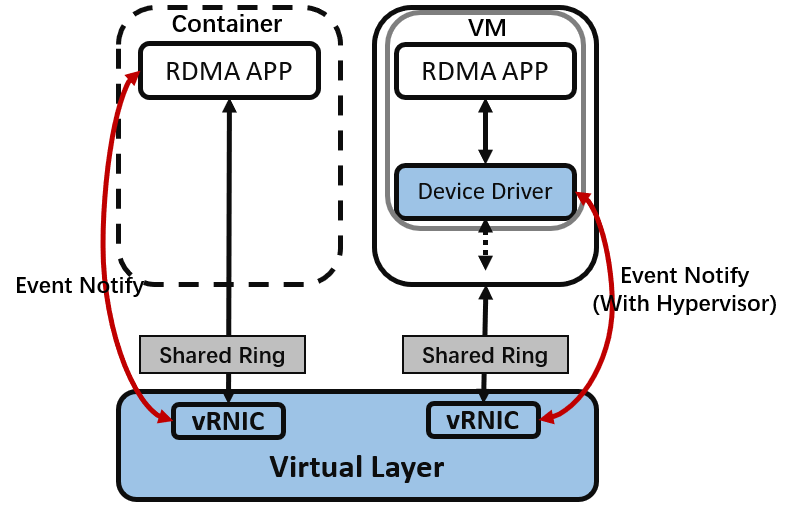
\includegraphics[width=1.0\linewidth]{images/interface-general}
	\caption{General uniVerbs Interface}
	\label{fig:interface-general}
\end{figure}


\item {\verb|Design the I/O device driver|}:
The goal of the device driver is to support I/O process inside each guest. As shown in in Figure~\ref{fig:interface-general},  the commands of RDMA application be forwared into the memory-shared queue, and trigger events to notify the vRNIC to process them; similarly, the device driver receives interrupt notifications and reads the result from vRNIC. In short, the device driver can be implemented by a lightweight kernel module.

\end{itemize}

 For generality, As shown in in Figure~\ref{fig:interface-general}, the same design as virtual machines is adopted for containers: in I/O channel, the file-based shared queue is also used; in the synchronization mechanism, the same event notification mechanism is used. But remind the container does not fall into the monitor or inject interrupts during the synchronization.

When there are multiple virtual machines or containers, if the files of each vRNIC are not isolated, they can be discovered by every container through scanning files. In order to solve this problem, we runs the virtual machine in a isolated container environment. Based on the container's mount namespace, we respectively place the shared files of each vRNIC in the dedicated directories and mounts each directory to the corresponding container(including containers running virtual machines). As a result, due to the isolation of the mount namespace, the shared files of each vRNIC in the virtualization layer are only visible to the used container or virtual machine.  

\begin{figure}[!ht]
	\centering
	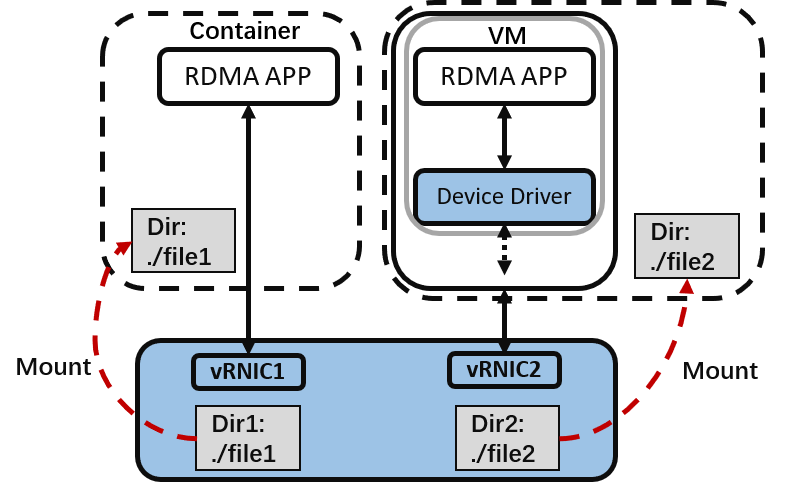
\includegraphics[width=1.0\linewidth]{images/interface-isolate}
	\caption{General uniVerbs Interface}
	\label{fig:interface-isolate}
\end{figure}

\subsection{uniVerbs Interface Optimization}
After completing the interface construction, the requests of RDMA applications can be transmitted to vRNICs, and the results can also be returned to the applications. In uniVerbs, zero copy of data and bypassing the virtual layer are realized by mapping the RDMA resources to vRNIC. As a result, data commands do not need to be forward to the virtual layer and this mode is consistent with native RDMA.

(1) zero copy optimization
The zero copy contents are including the RDMA work request in the QP queue and the transfer data in the registered memory, and the process is from RDMA application to pyhiscal RNIC. Remind that vRNIC RDMA resources are mapped to VFs, so we only need to make sure the zero-copy from RDMA application to vRNIC.

The fact of zero-copy is that both processes have common availiable physical memory pages. Similar as the above I/O channels, file-based shared memory are also used when mapping QP and other RDMA resouces and this is general for both virtual machines and containers.

\begin{figure}[!ht]
	\centering
	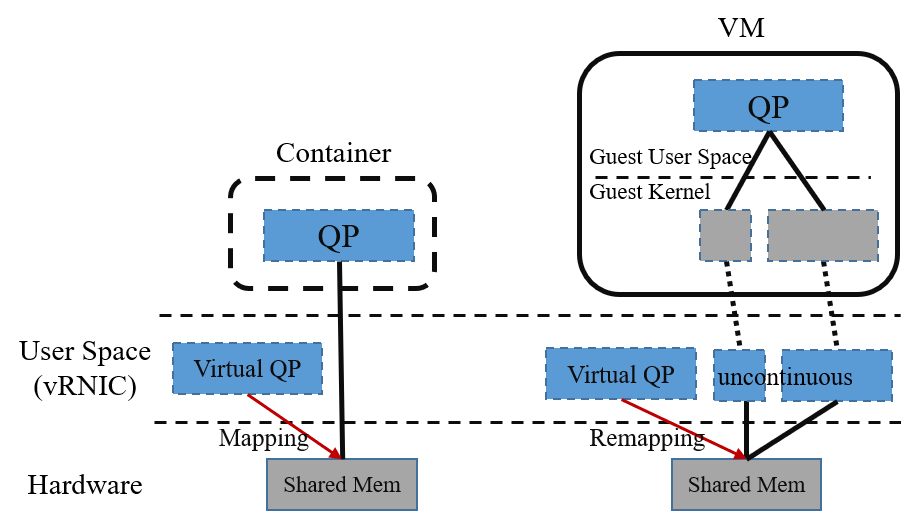
\includegraphics[width=1.0\linewidth]{images/zero-copy}
	\caption{Mapping QP to vRNIC}
	\label{fig:zero-copy}
\end{figure}

However, in the virtual machine, due to the memory management mechanism of guest operating system, the virtual machine's physical memory of the RDMA resource may be not continuous, and the mapped memory area in vRNIC is not continuous. So, vRNIC can not map the virtual memory area as a virtual RDMA resource to RNIC. To solve this problem, the virtual memory remapping mechanism in user space is used. It remaps the discontinuous RDMA resource virtual memory area in vRNIC to the a block of continuous virtual memory, and the  sequence of mapped physical memory page must be unchanged.

(2) Bypassing virtual layer optimization
Pressing the doorbell is necessary in RDMA data path to drive RNIC. In vRNIC, the doorbell that is mapped to VF, still need to be mapped to RDMA application tp meet bypassing. Otherwise, the pressing command needs be forward to vRNIC and thats imports apperant latency in data path.

However, the RDMA application and the vRNIC belong to two different processes on the host, and they have isolated virtual address spaces. At the same time, the doorbell register is located in the device address space and cannot be mapped by shared memory. The key to solving this problem is that the process of RDMA application needs to know the physical address of the doorbell register.

\begin{figure}[!ht]
	\centering
	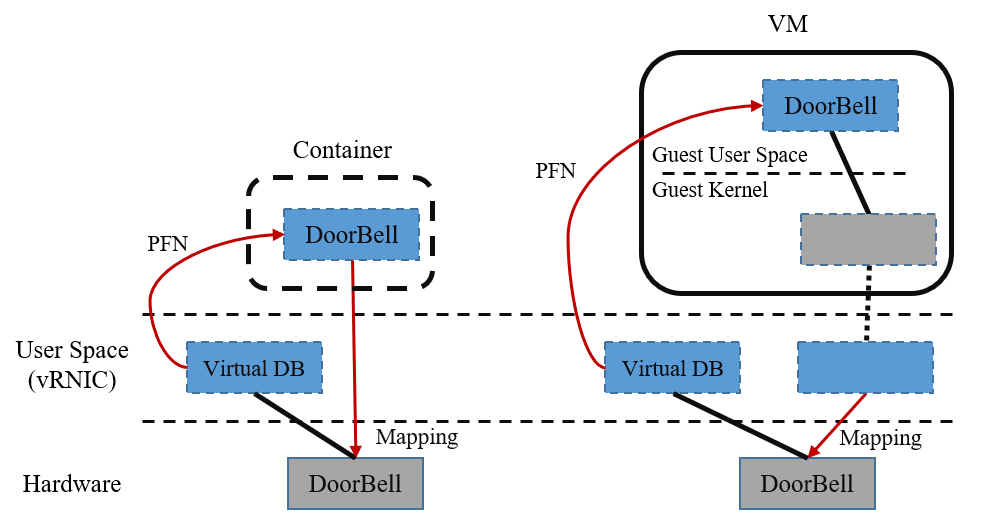
\includegraphics[width=1.0\linewidth]{images/by-pass}
	\caption{Mapping DB from vRNIC}
	\label{fig:by-pass}
\end{figure}

Therefore, when an RDMA application creates a RDMA context, it sends a request to the vRNIC at first. Under the supervision of virtual layer, vRNIC forwared to application with the corresponding physical address of the doorbell, commonly the physical page number. After that, the application maps its doorbell virtual address to the physical page in its own process, that needs the host kernel and hypervisor if the application in virtual machines.

